\documentclass[11pt]{article}
\usepackage{graphicx} % Required for inserting images
\usepackage{amsmath}
\usepackage[natbibapa]{apacite}
\usepackage{natbib}
\usepackage{setspace}

\begin{document}
\begin{titlepage}
    \begin{center}
        \vspace*{1cm}
        
        \Large
        \textbf{Gompertz model out-perform logistic and linear models for quantifying bacterial grwoth data}
        
        \vspace{1.5cm}
        
        \textbf{ZhongbinHu}\\
        Affiliation: Imperial College London\\
        Email: zh1323@ic.ac.uk
        
        \vfill
        
        Word Count: 2934 words
        
        \vspace{0.8cm}
        
        \Large
        Date: 2 Dec 2023
        
    \end{center}
\end{titlepage}


\onehalfspacing
\section{Abstract}
This study aims to compare the effectiveness of logistic and Gompertz models against quadratic and cubic models in capturing the growth patterns of diverse bacterial species.  Utilizing data from global lab experiments, we employed statistical measures like Akaike Information Criterion (AIC), Bayesian Information Criterion (BIC), and R-squared to assess model fit.

My methodology involved fitting each model to bacterial growth data, with a focus on initial parameter estimation for enhancing model accuracy.  The results revealed that non-linear models, particularly the Gompertz model, provided a superior fit across most species, as indicated by lower AIC and BIC values compared to linear models.  This superiority was attributed to the Gompertz model's ability to encapsulate the lag phase of growth, a critical phase often inadequately represented in linear models.
\section{Introduction}
Bacteria are one of the most abundant and diverse groups of microbes on Earth, and the growth and abundance of them plays a vital role in the ecosystem. Bacteria can contribute to the global carbon cycle through reactions such as photosynthesis. At the same time, bacteria can promote the transfer of nutrients by breaking down organic matter, thus supporting the productivity of the entire ecosystem\cite{keller2006}. The population growth rate of bacteria also plays an important role in medicine and public health, and the rapid reproduction of bacteria can lead to the rapid spread of diseases. The growth of bacterial resistance is also closely related to the dynamics of bacterial populations\cite{rivera-tapia2003}. Understanding and predicting the growth patterns of bacterial populations is critical to developing effective disease control strategies.

Predictive microbiology was proposed by Roberts and Jarvis
\cite{ross2003}, The goal of predictive microbiology, is to develop a mathematic equation which describes the behavior of microbes \cite{md2011}. Central to this endeavor is the employment of models to interpret the growth patterns of microbial populations, particularly bacteria. The concept, these models range from mechanistic theories, grounded in the principles of population dynamics and resource availability, to phenomenological approaches that empirically describe observed growth patterns without delving into underlying biological mechanisms. 


At the heart of population growth models is the Malthusian principle\cite{mcatee1936}, which posits that populations expand exponentially in the absence of resource limitations. However, real-world scenarios often deviate from this simplicity. As resources become scarce, growth rates decelerate, eventually stabilizing as populations reach the carrying capacity of their environment. This complex interplay of growth, resource utilization, and environmental constraints is conspicuously evident in bacterial populations. Bacteria, with their rapid growth rates and sensitivity to environmental changes, serve as ideal subjects for studying population dynamics.

Overall, the models primarily describe and predict microbial growth in "closed habitats." In a "completely enclosed habitat," all life-sustaining resources are limited and non-renewable, while metabolites excreted by living cells and dead cells are not removed \cite{peleg2011}. There are four distinct stages of typical growth in enclosed habitats, namely the “lag phase” where cells acclimatize and prepare for growth, “exponential growth phase,” characterized by rapid, a “stationary phase,” where growth plateaus as resource limits are reached, and a “mortality phase”\cite{peleg2011}. In most of microbiology cases, mortality phase is not included in the model. However, these methods offer a limited view, prompting the development of more comprehensive models that encapsulate the sigmoidal growth curve of bacterial populations.



In this context, my study aims to critically analyze and compare different mathematical models applied to microbial population growth data across species. I explore how well mechanistic and phenomenological describes the complexities of microbial growth. Four models were used in this project, which are quadratic, cubic, logistic and Gompertz models. AIC and BIC value were applied to evaluate model fitting. In this project, I am trying to find: 1. Is non-linear model fits better than linear model? 2.is Gompertz model fits better than logistic model?

\section{Method}
\subsection{Computing Languages and tools}
R is a programming language designed for statistical analysis and graphical representation, with toolkits such as minpack.lm for ease of use.
R provides powerful graphics and visualization tools, such as the ggplot2 package, that help me present complex data and analysis results in a more intuitive way. 
At the same time, such as dplyr, reader and other toolkits are convenient for processing datareadr: Used to load data. 
dplyr: Data processing and cleaning. I used functions to process the data, such as creating unique ids, deleting NA values and negative values.
minpack.lm: Contains the nlsLM function, which is a more robust nonlinear least squares fitting function for fitting logistic and Gompertz models.
broom: Used to organize the output of model fitting. The glance function extracts the overall statistics of the model, such as R-squared, AIC, and BIC.
ggplot2: Generates a chart. I used ggplot to visualize raw data points and fitted curves for different models.

\subsection{Data}
The data used in this project were collected from lab experiments all over the world.The data shows the bacterial population in given time of different bacterial species.

\subsection{Models}

I used quadratic and cubic polynomial model . The two models are similar. Cubic models are more complex and flexible than quadratic models, but this can also lead to problems with overfitting. Compared to simple linear models, Quadratic and cubic models provide greater flexibility and can accommodate more complex data structures\cite{penny2011}. 
They are effective tools for exploring patterns in the data. Especially in cases where the data is insufficient to support more complex models, quadratic and cubic models can serve as phenomenological methods that provide a basic understanding of data trends. It is applicable when the data show an approximate linear relationship\cite{penny2011}. When microbial population growth is close to linear in the observed time window, a linear model is appropriate and easy to explain. This is often seen in a particular phase of population growth, such as the exponential growth phase. Because of its simplicity, the linear model can be easily applied to different types of microbes.

A classical (somewhat) mechanistic model is the logistic equation\cite{zwietering1990} .The sigmoidal curve produced by the logistic model is well suited to describe population growth under resource constraints. It starts with slow growth, accelerates as resources are used, and eventually slows as resources are depleted. The effects of resource constraints on population growth are considered. At the same time, the parameters in the model are also of ecological significance, which makes the model have a good explanation in biology.:
\begin{equation}
    N(t) = \frac{N_0 \times K \times \exp(r_{\text{max}} \times t)}{K + N_0 \times (\exp(r_{\text{max}} \times t) - 1)}
\end{equation}
where the parameters represent:
\begin{itemize}
    \item $N(t)$: The population size at time $t$.
    \item $N_0$: The initial population size.
    \item $K$: The carrying capacity of the environment, which is the maximum population size that the environment can sustain.
    \item $r_{\text{max}}$: The maximum rate of growth of the population.
\end{itemize}
Here Nt is population size at time t, N0 is initial population size, r is maximum growth rate (rmax), and K is carrying capacity (maximum possible abundance of the population).


It is similar in form to the logistic model, but provides different shapes of the growth curve, Better description of the early stages of population growth, especially if the rate of growth is gradually increasing\cite{zwietering1990}. Compared to the Logistic model, the Gompertz model provides greater flexibility and complements in describing specific stages of population growth, especially initial and final stages
\begin{equation}
    N(t) = N_0 + (K - N_0) \times \exp\left(-\exp\left(r_{\text{max}} \times e \times \frac{t_{\text{lag}} - t}{(K - N_0) \times \log(10)} + 1\right)\right)
\end{equation}
where the parameters represent:
\begin{itemize}
    \item $N(t)$: The population size at time $t$.
    \item $N_0$: The initial population size at the beginning of the observation period (at $t = 0$).
    \item $K$: The environmental carrying capacity, which is the maximum population size that the environment can sustain.
    \item $r_{\text{max}}$: The maximum growth rate, representing the fastest growth speed of the population.
    \item $t_{\text{lag}}$: The lag time, which is the delay before the population starts to grow significantly.
    \item $e$: The base of the natural logarithm is approximately equal to 2.71828.
\end{itemize}

\subsection{Starting values}
t-lag represents the time of from the start to the end of time-lag phase. Based on finding the point at which population growth accelerated, t-lag can be calculated. 

Mas growth rate is considered as a measure of species population growth intensity. Max growth rate is the largest gradient in the curve. In this project, rolling regression was used to find the largest growth rate.

The initial number, which is N0, represents the population at the start point. in Gompertz model N0 in log scale was used, which might reduce the experimental error\cite{peleg2011}. In this project, it was the minimum population as the start population. This selection assumes that the smallest value in the observed data set is close to the initial population size.

Asymptotic Growth Level is defined as the population of “stationary phase” which represents the carrying capacity of the environment\cite{peleg2011}. In this project, Asymptotic Growth Level was the largest population in the data. This selection assumes that the largest value in the observed data set is close to the varying capacity.

Using different models can provide different perspectives on bacterial growth dynamics. For example, linear models may capture certain characteristics of the data, while Logistic and Gompertz models are more reflective of biological processes and population dynamics.

\subsection{Modelling fitting}
Model selection is considered as one the most reliable way to find the best fitted model. 
Three statistical methods are often used, 1. maximizing fit; 2. null hypothesis tests; 3. model selection criteria\cite{johnson2004}.  Finding the model that maximizes a fit measure, like adjusted R2. 
When prioritising the best fit, it fails to consider the principle of parsimony and, as a result, may lead to inaccurate parameter estimations and forecasts, rendering it an inadequate method for model selection. On the other hand, tests or criteria that consider both suitability and complexity are more appropriate for choosing a model.
The likelihood ratio test (LRT) is the most employed method for testing null hypotheses. Nevertheless, it is not possible to utilise any type of likelihood ratio test (LRT) to measure the comparative level of support between competing models.
Model selection criteria evaluate the goodness of fit and complexity of different models, such as AIC, BIC allowing for the comparison of numerous models at the same time. 
Many researchers are transitioning from likelihood ratio tests (LRTs) to model selection criteria when considering fit and model complexity\cite{posada2003}. 
\begin{itemize}
    \item \textbf{AIC (Akaike Information Criterion)}: 
    A measure of the relative quality of a statistical model for a given set of data. It is defined as:
    \begin{equation}
        \text{AIC} = 2k - 2\ln(L)
    \end{equation}
    where $k$ is the number of parameters in the model, and $L$ is the maximized value of the likelihood function for the model.
    
    \item \textbf{BIC (Bayesian Information Criterion)}: 
    Similar to AIC, but with a different penalty for the number of parameters. It is defined as:
    \begin{equation}
        \text{BIC} = \ln(n)k - 2\ln(L)
    \end{equation}
    where $n$ is the number of data points, $k$ is the number of parameters, and $L$ is the likelihood of the model.
    
    \item \textbf{R Squared ($R^2$)}: 
    A statistical measure that represents the proportion of the variance for a dependent variable that's explained by an independent variable or variables in a regression model. It is defined as:
    \begin{equation}
        R^2 = 1 - \frac{\text{Sum of squares of residuals}}{\text{Total sum of squares}}
    \end{equation}
\end{itemize}

Therefore, Adjusted R2 is mainly used as a measure of fit.AIC represents the fit and complexity of the model.BIC includes fit, complexity and sample size.

\section{Results}
\begin{table}
    \centering
    \begin{tabular}{cccc}
         &  AIC&  BIC& R squared\\
         Quadratic model&  16.307&  17.731& 0.853\\
         Cubic model&  0.725&  2.624& 0.909\\
         Logistic model&  1.998&  3.395& 0.919\\
         Gompertz model&  -11.682&  -9.905& 0.954\\
    \end{tabular}
    \caption{the mean value of R squared, AIC and BIC of four models}
    \label{tab:my_label}
\end{table}

table 1 shows the mean vlaue of Rsquared, AIC, and BIC of four models. From table 1, the AIC and BIC of  Quadratic are quite large, while the values of the Gompertz model are quit low., which means the Gompertz model fits the data the best.
\begin{table}
    \centering
    \begin{tabular}{ccccc}
         Models&  Quadratic&  Cubic&  Logistic& Gompertz\\
         Counts&  21&  50&  82& 129\\
    \end{tabular}
    \caption{The number best models fitting different species based on AIC}
    \label{tab:my_label}
\end{table}

From table 2, Gompertz model is the best fitting model in most of the species (129). The logistic equation fits 82 models the best. And total number of linear models is smaller than non-linear model. The cubic model fits 50 species as the best model, while the quadratic only fits about 21 sub-data sets.
\begin{table}
    \centering
    \begin{tabular}{ccccc}
         Models&  Quadratic&  Cubic&  Logistic& Gompertz\\
         Counts&  21&  50&  85& 129\\
    \end{tabular}
    \caption{The number best models fitting different species based on BIC}
    \label{tab:my_label}
\end{table}

From the BIC table 3, the result is quite similar to  table 2. Gompertz model is the best fitting model in most of the species (129). The logistic equation fits 85 models the best. And total number of linear models is smaller than non-linear model. Cubic model fits 50 species as the best model while Quadratic only fits about 21 sub-data set.


\section{Discussion}
\subsection{Comparing different models}
\begin{figure}
    \centering
    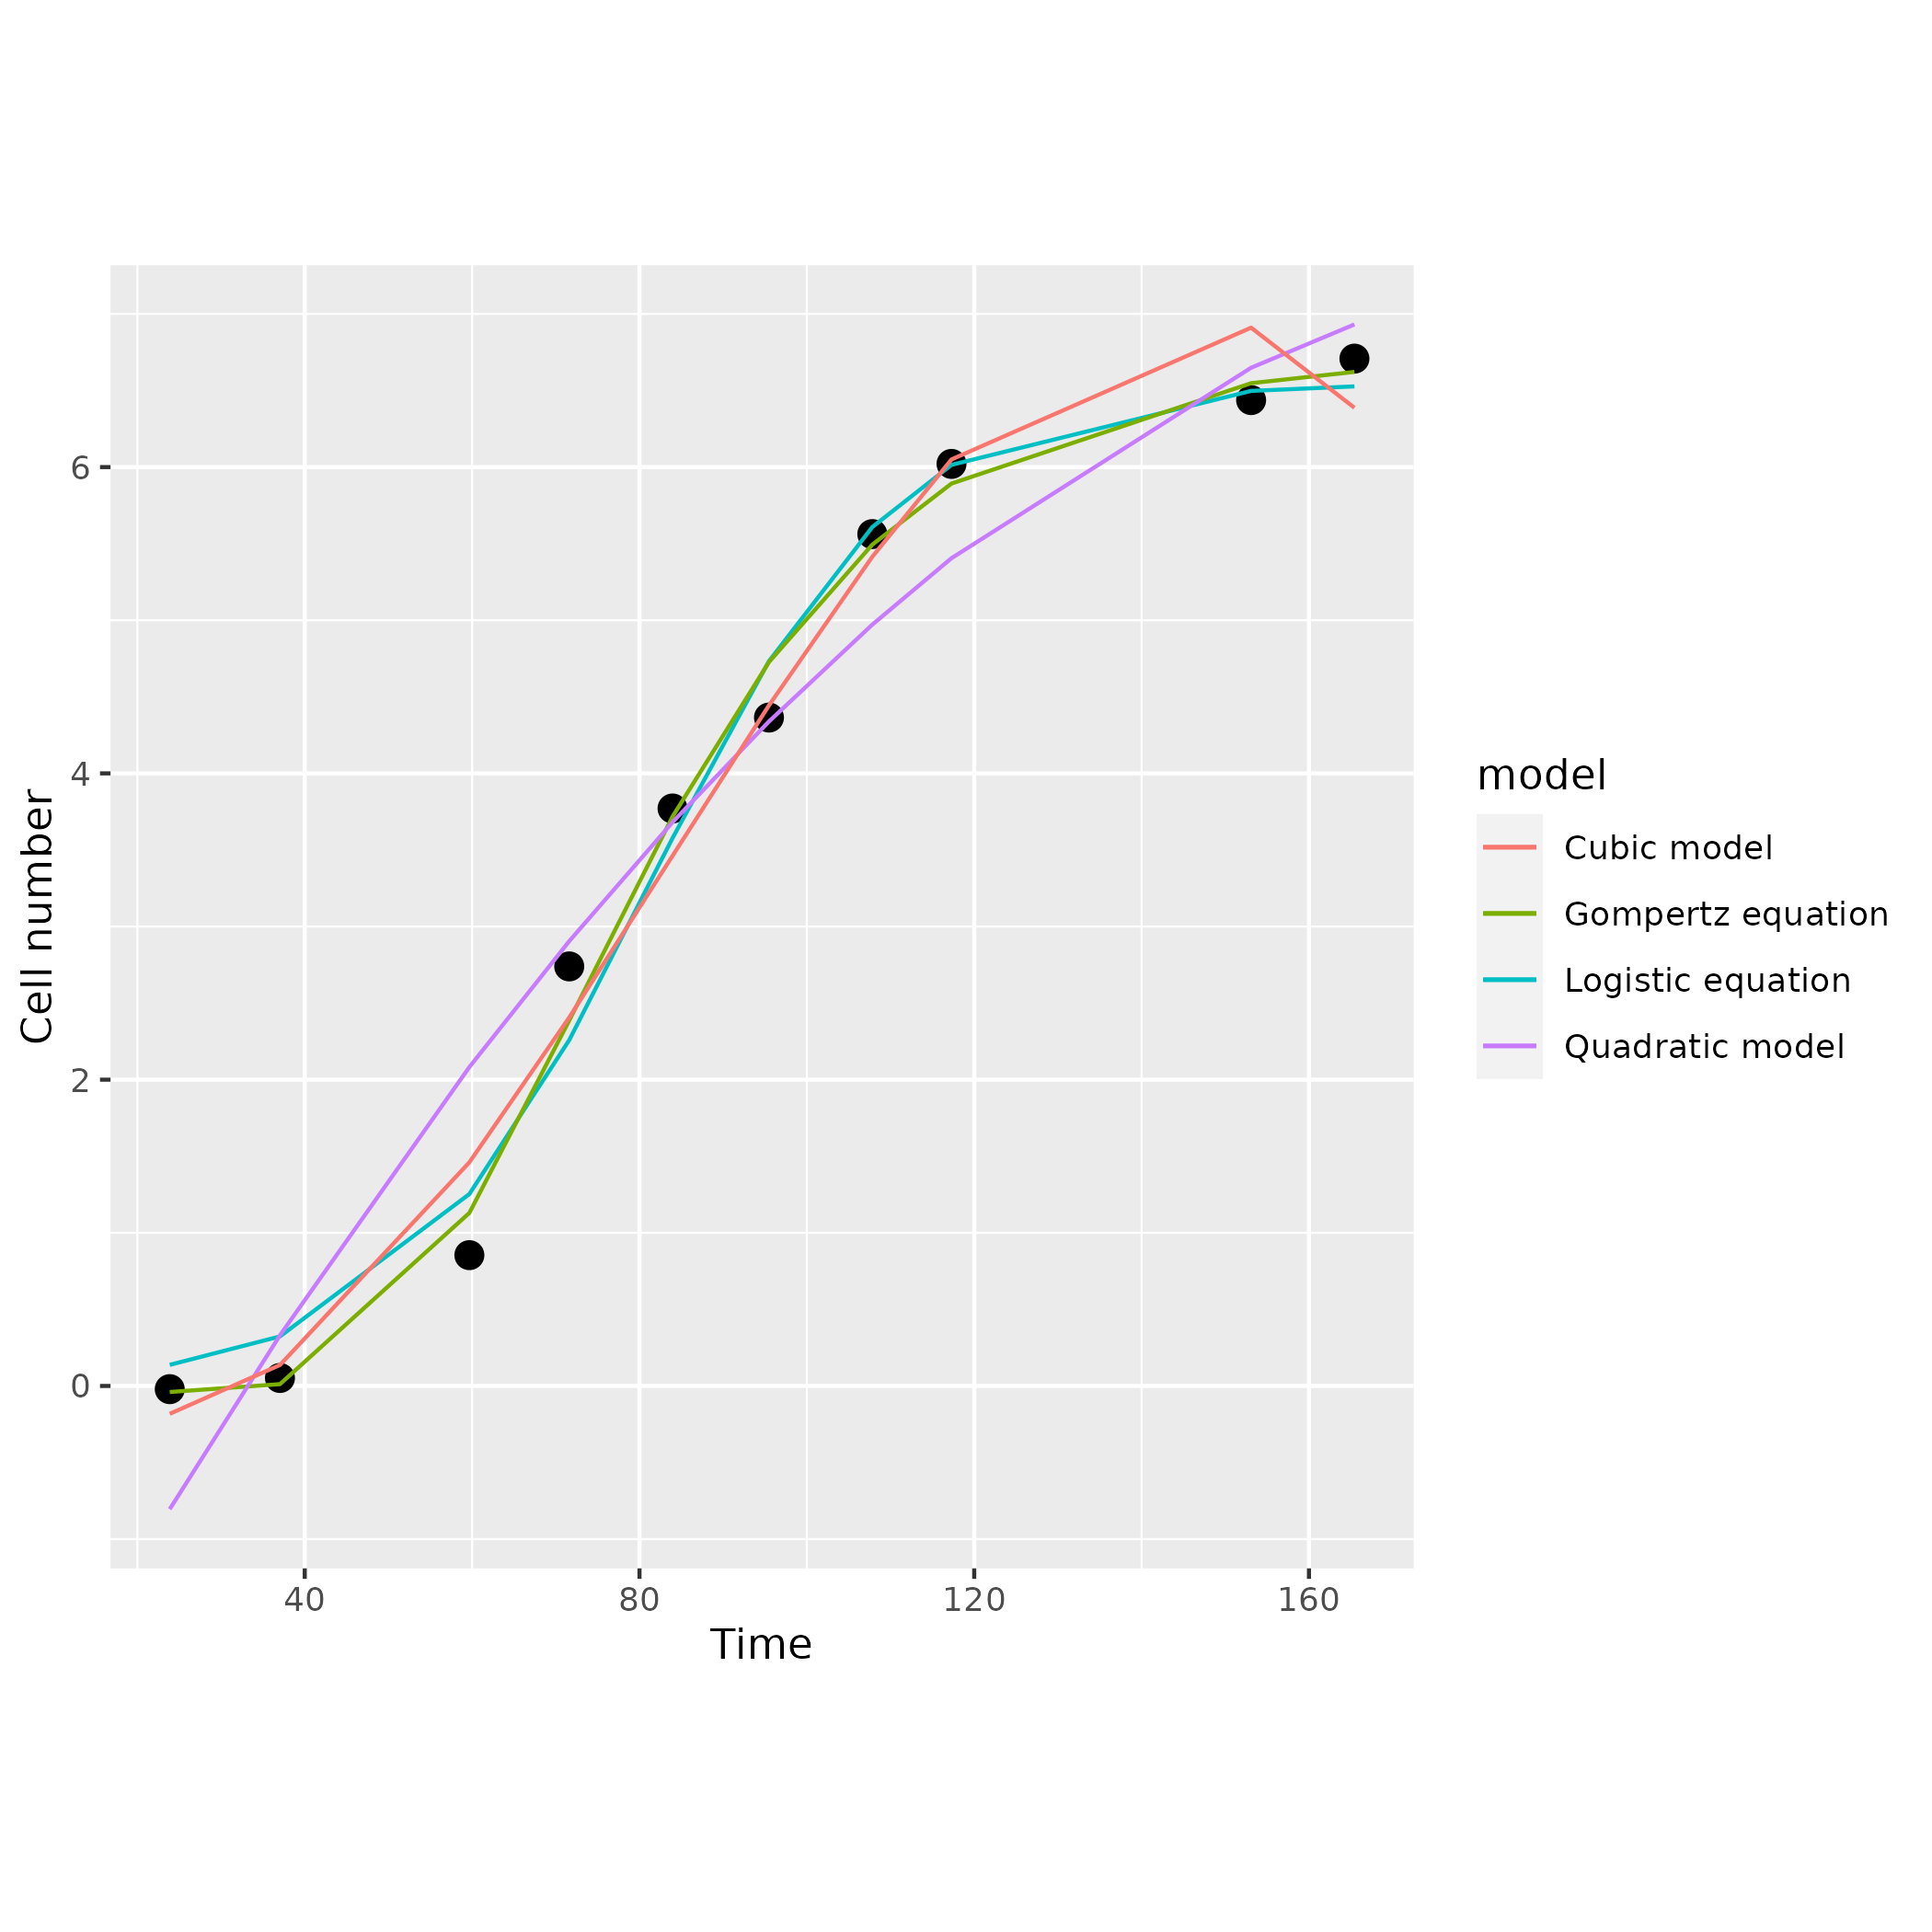
\includegraphics[width=0.5\linewidth]{../results/subset_ 14 _plot.png}
    \caption{the plot of subset data 14}
    \label{fig:subset1-plot14}
\end{figure}

From table 2 and 3, the non-linear model fits better than linear model.Biological processes, especially those like bacterial growth, often exhibit nonlinear characteristics. For example, bacterial growth tends to be slow at first, then rapidly increases, and finally slows down as resources are depleted, eventually reaching a stable state. Nonlinear models often provide parameters that are more directly related to biological processes\cite{zwietering1990} (such as growth rate, carrying capacity, etc.) that have clear biological significance.The parameters of a linear model may be difficult to relate directly to specific biological features.
This sigmoid curve (population grwoth curve) is a typical nonlinear behavior, which is the majority of curves in the data (Figure 1).  Sincce the data points represent the growth process from the "time-lag phase " to the "stationary pahse". Gompertz's model fits the curves the best. 
Some of the data subset didn't contain "time-lag" phases(shown in figure.2) In this case, the logistic model fits the data the best.
\begin{figure}
        \centering
        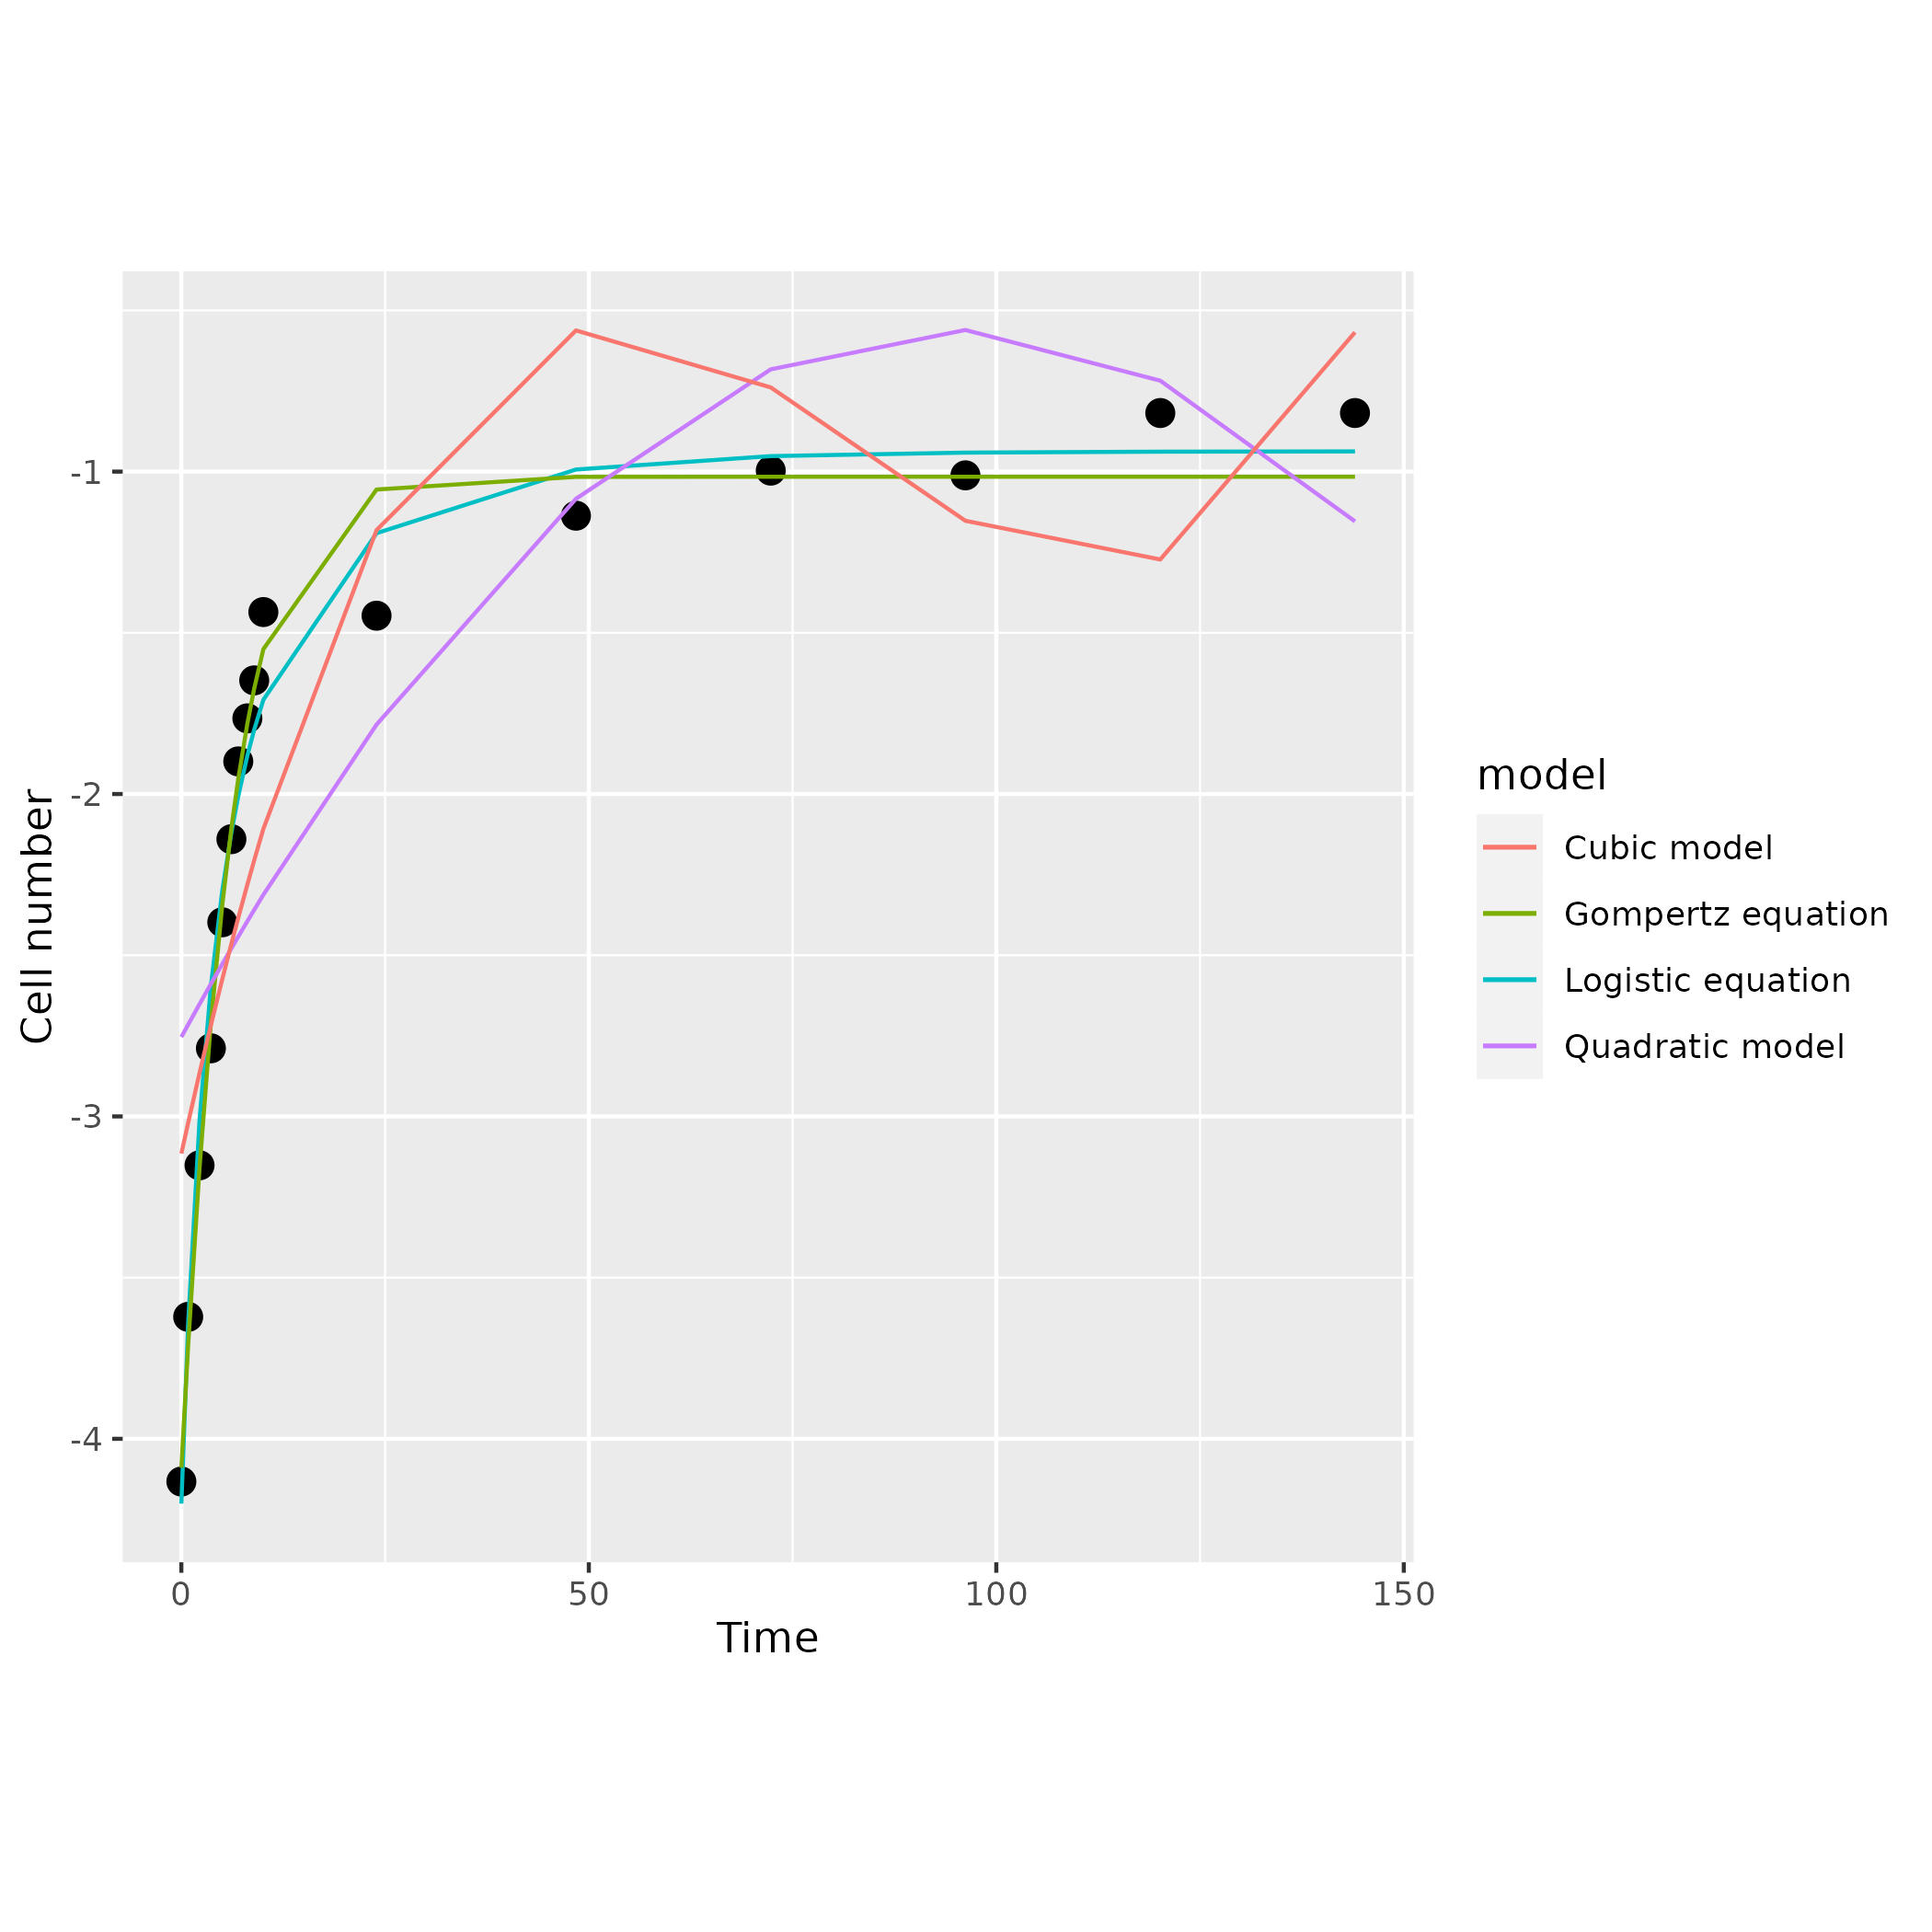
\includegraphics[width=0.5\linewidth]{../results/subset_ 7 _plot.png}
        \caption{the plot of subset data 7 }
        \label{fig:subset1-plot7}
    \end{figure}

Linear models, due to their simplicity, may have a strong ability to describe data with simple trends. Some of the data subset may only includes "exponential phases"(shown in figure 3). Quadratic model becomes the best model fitting the data. In figure 4, the population size drops instead of keeping steady. this might because, the bacteria enter "mortality phase". Both logistic and Gompertz model could not fit the data well. Cubic model becomes the best model in this data subset.
\begin{figure}
    \centering
    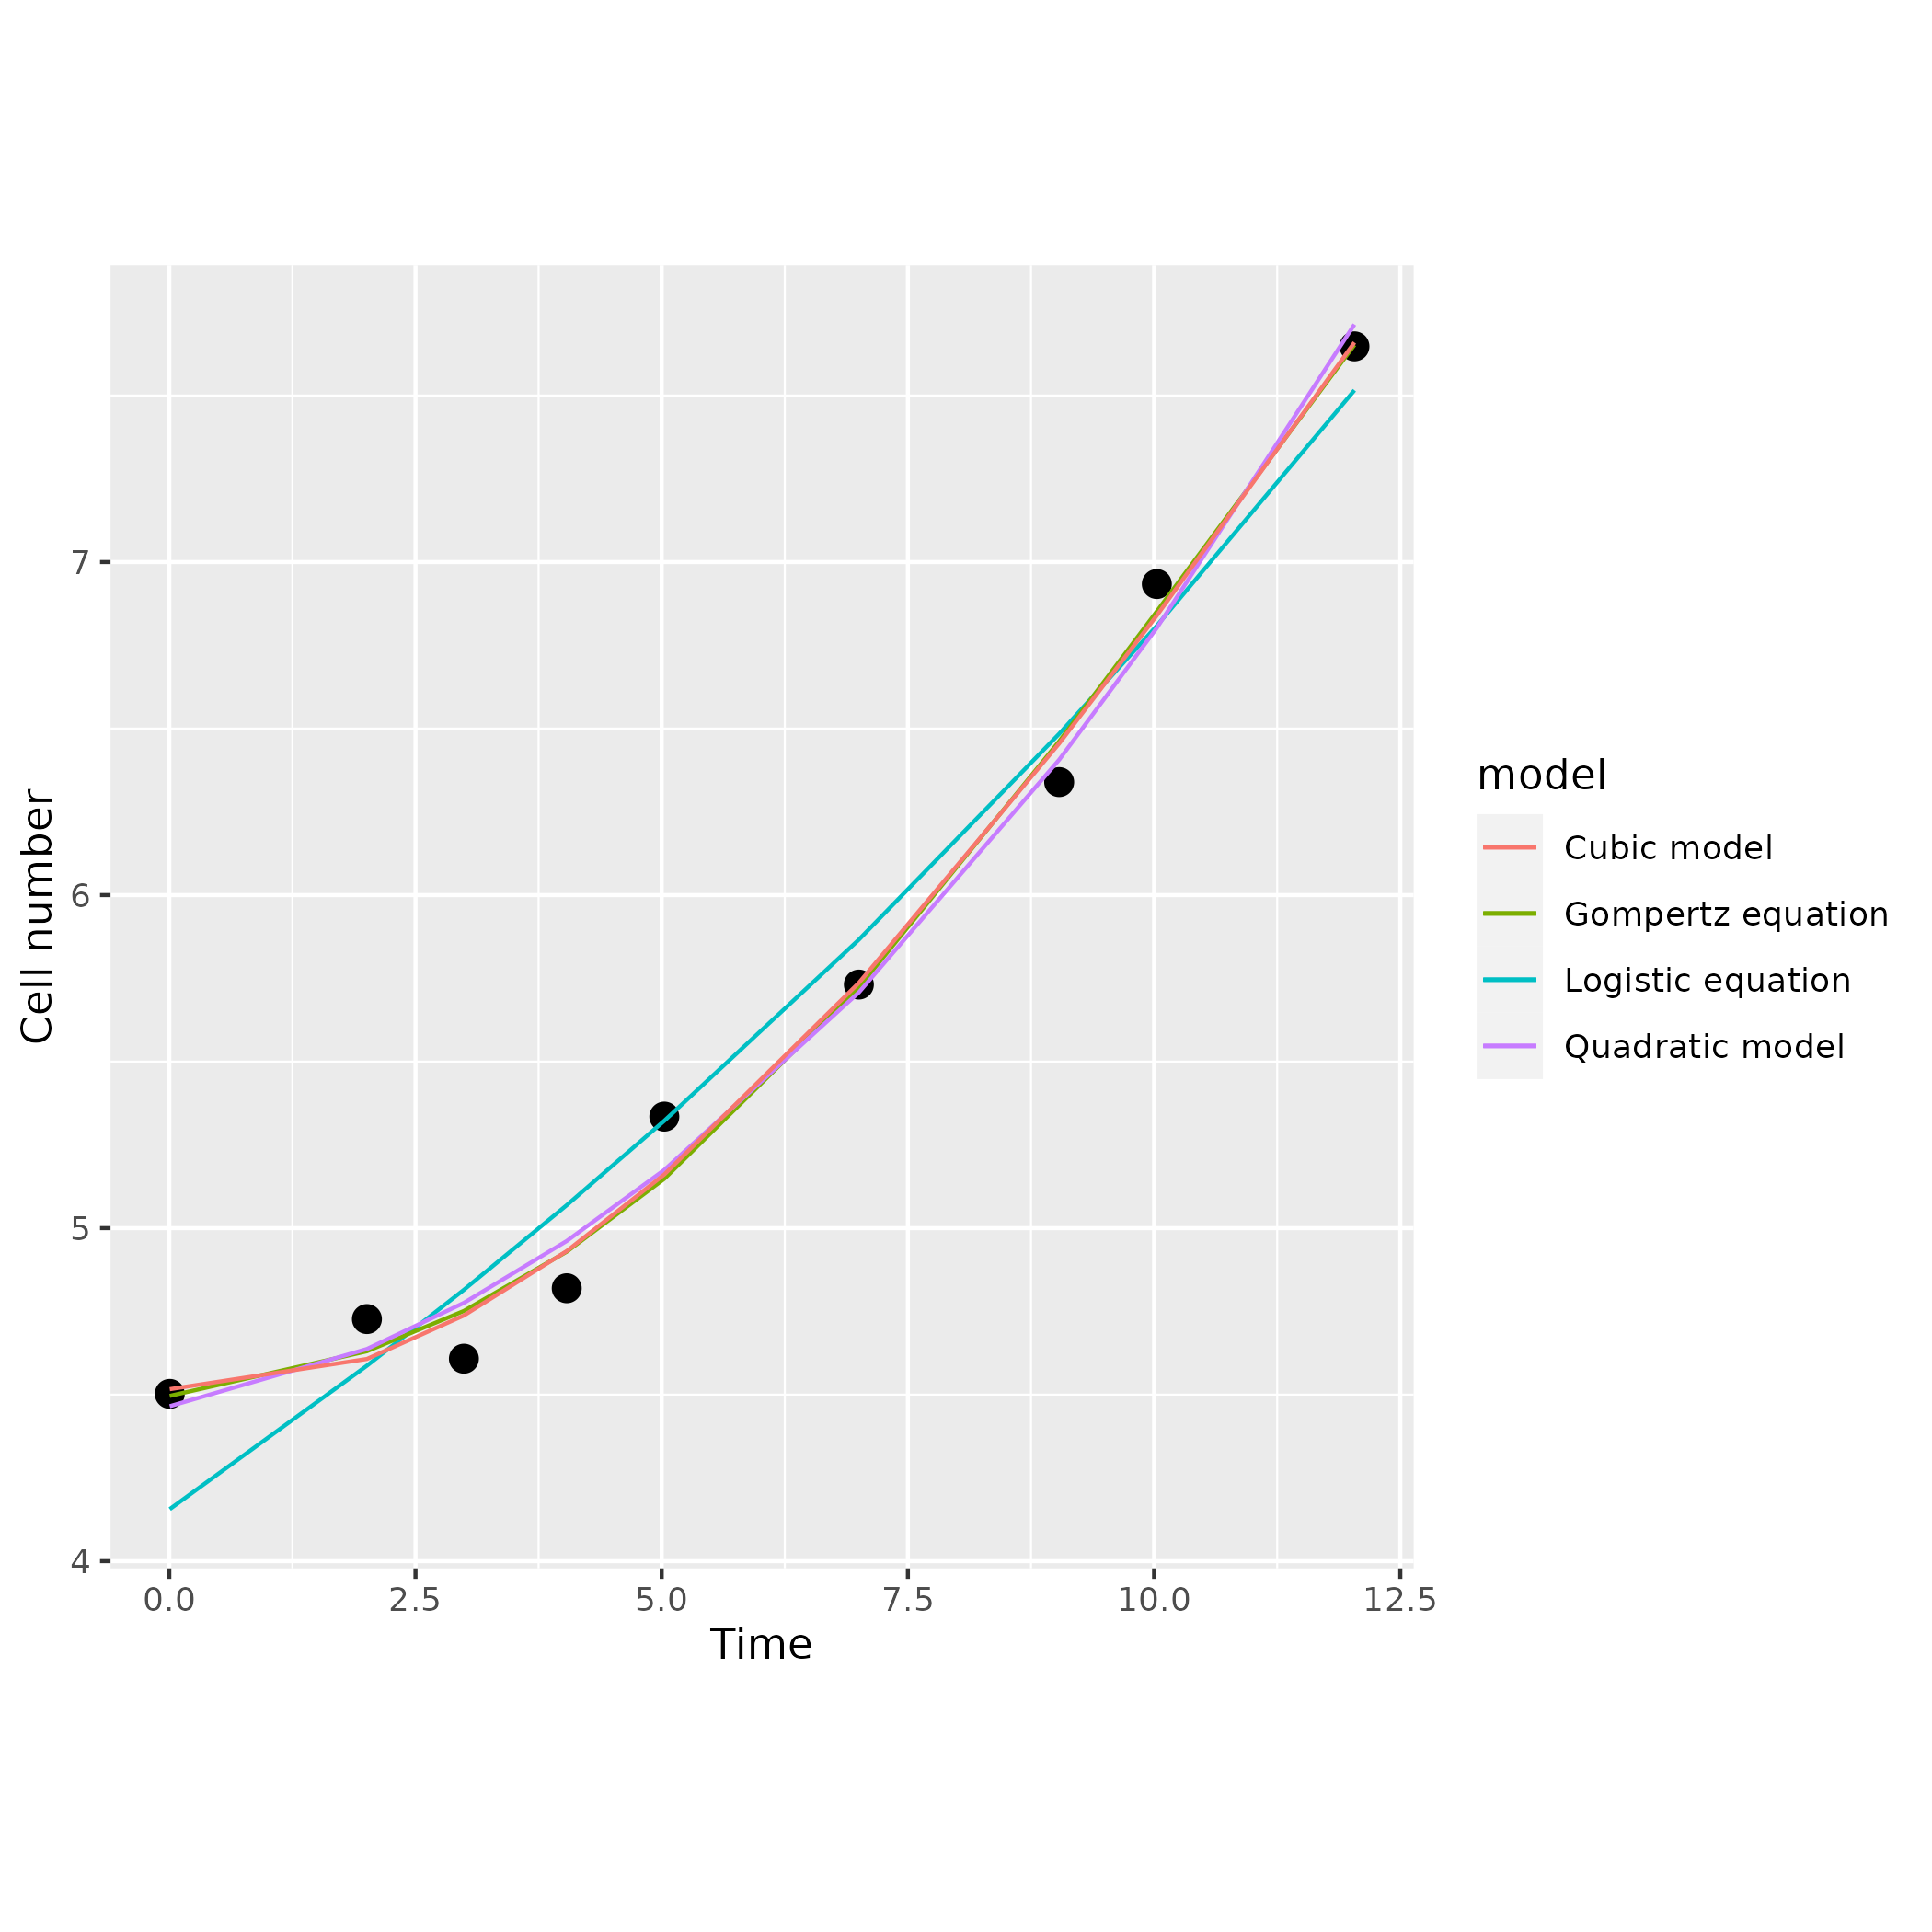
\includegraphics[width=0.5\linewidth]{../results/subset_ 116 _plot.png}
    \caption{the plot of subset data 116}
    \label{fig:subset1-plot116}
\end{figure}

\begin{figure}
  \centering
    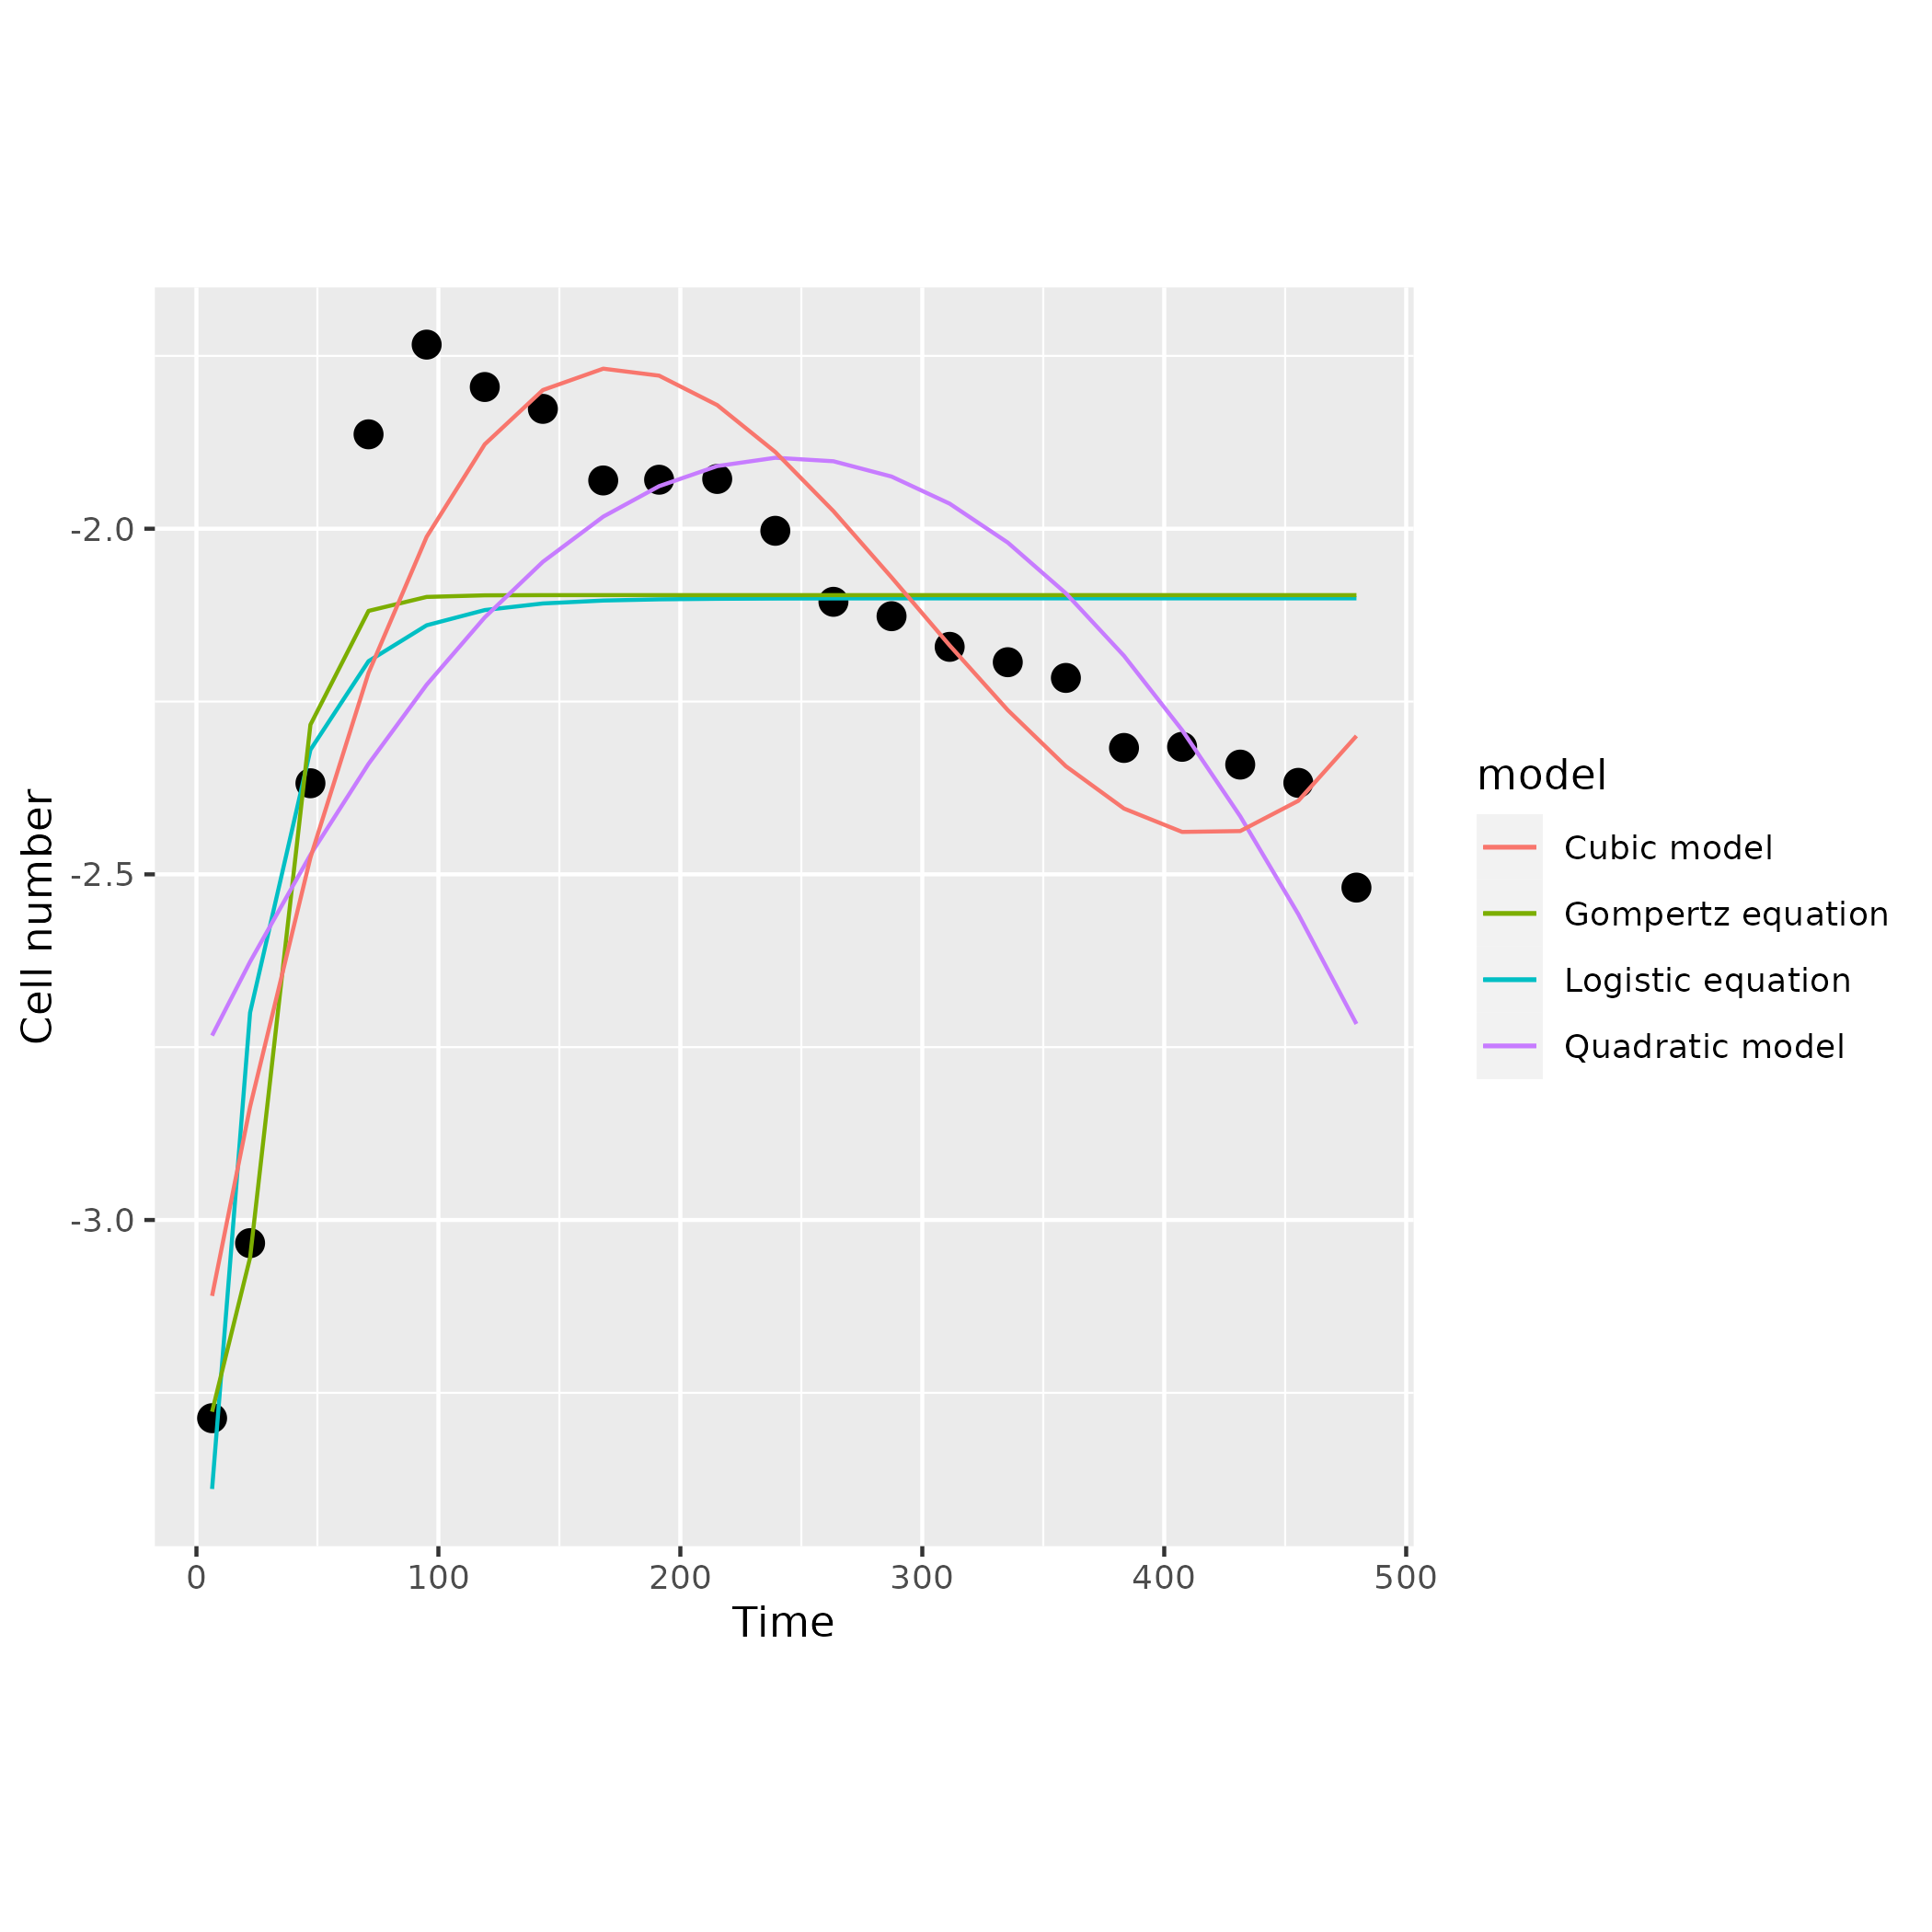
\includegraphics[width=0.5\linewidth]{../results/subset_ 1 _plot.png}
    \caption{the plot of subset data 1 }
    \label{fig:subset1-plot1}
\end{figure}

From the result, Gompertz might be the best model fitting bacterial population growth.In the real world, it takes time for microbes to grow. Therefore, a time lag before exponential growth is needed. Gompertz model contains t-lag as the parameter, which means it might be more accurate and complete than logistic model. 

However, Gompertz model could not fit all the subsets. In some cases, the linear model becomes the best model. this might because, the time of a complete stages of population growth is unknown, the data might only demonstrate part of phases. For example, the linear model could fit the exponential stage quite well. Therefore, in some of the data subsets, linear model might be the best fitted model. 

\subsection{number of parameters}
The number of parameters in models may also influence the result. The increased number of parameters may lead to increasing of model complexity, which might contribute the models to capture more complex mechanisms. However, Occam’s rzzor principle suggests that the simple one is preferred when comparing two models\cite{domingos1999}. More parameters in models might cause over-fitting, which means the model may not fit new data\cite{domingos1999}. In addition, more parameters may require more explanations, bring about difficulties in explaining the model. The balance between the number of parameters is quite important in models. 

\subsection{starting values}
Starting values may affect the model quality. From the R results, there are about 30 Gompertz models is NA., which also contains the most NAs among the models. This might because of the limitations of starting values.

There is not clearly definition of the duration of lag-time since the transition from the slow growth to exponential growth rate is continuous instead of sudden \cite{peleg2011}. There are two ways to find the lag-time, one is to find the across point s visually, and the other is to include t-lag in a non-linear model\cite{mckellar2003}. However, there might be potential problems., since it is hard to be sure about t-lag value. This means their might be errors in model fitting by using t-lag. In theory, even for growth curves with a lengthy "lag time," A can only be approximately equal to log N0 due to the fact that the second term on the right side of the equation never reaches an exact value of zero. Converting a model to a rate model for predicting dynamic growth might pose a significant challenge when describing the boundary condition. .

 As for the Asymptotic Growth Level, if the clear stationary phase does not occur, then the asymptotic value will just be an extrapolated value\cite{peleg2011}. Therefore, the value might not represent the reality condition. 


\subsection{Model selection}
In the case of a large sample size, the BIC may prefer a more concise model with fewer parameters, even if the model's prediction accuracy is slightly improved. This is because the BIC penalty increases as the sample size increases, making overly complex models subject to stricter penalties due to the increased number of parameters\cite{kuha2004}. Therefore, on large data sets, using BIC as the model selection criterion can effectively avoid the problem of over-fitting.This might explain why the number of Gompertz models decreases in the table when applying BIC.


By comparing the models, it can be found it is significant to assign the parameters in models’ different meanings. From Gompertz model, t-lag is one of the most important parameters in population growth. The results also show that t-lag is significant. in addition, choosing an appropriate model is also important in simulating population growth. Different models equations may lead to large difference in results. 

\subsection{limitations}
To make sure all the models can be compared to each other. LogN is used instead of N.This might cause larger residuals compared to the actual population.
Varying statistical fit criteria may produce disparate outcomes due to the presence of outliers. Furthermore, it is crucial to note that the experiment's duration may be limited due to logistical or other constraints. As a result, the microbial level in the stored food could potentially exceed the model's predictions through extrapolation. Additionally, it is possible that the microbial level may not stabilise if mortality occurs\cite{peleg2011}. 
Due to the log scale, the discrepancy between fitted value and true value may also increase. Unless the experimental growth data has hit a plateau, the regression technique may be unstable. Starting with varied initial predicted values can lead to varying growth parameters or the iterations failing to converge.There is negative data which was removed, since the negative data can not be used in model fitting.

No models include "mortality phase" of  population growth. all the phases in the growth process may be significant to be studied. it contributes to controlling bacterial growth by knowing the complete process of population growth. more parameters is required to explain the mortality phases in model.

\subsection{summary}
The primary objective of our study was to analyze the growth dynamics of various bacterial populations by applying logistic and Gompertz models. Utilizing Akaike Information Criterion (AIC), Bayesian Information Criterion (BIC) and R squared as measure of fit to assess the relative merits of the models, we observed that the Gompertz model generally provided a better fit, although in some cases the logistic model was more appropriate. In addition, non-linear model fits population growth better than linear model. Their performance might be significantly influenced by the data, parameters, and other ecological factors. 

\newpage  
\bibliographystyle{apacite}
\bibliographystyle{apalike} 
\bibliography{miniproject.bib}
\end{document}
